\documentclass[11pt,a4paper]{article}

\usepackage[margin=1in]{geometry}
\usepackage{graphicx}
\usepackage{booktabs}
\usepackage{hyperref}
\usepackage{amsmath}
\usepackage{caption}
\usepackage{subcaption}
% natbib removed; using basic \cite with thebibliography
\usepackage{xcolor}
\usepackage{enumitem}
\usepackage{float}
\usepackage{tikz}
\usetikzlibrary{shapes.geometric, arrows.meta, positioning, calc}

\hypersetup{
    colorlinks=true,
    linkcolor=blue,
    citecolor=blue,
    urlcolor=blue,
}

\title{\textbf{Are You in the Simcluster?}\\[6pt]
\large A Diagnostic, Philosophical, and Mildly Uncomfortable Guide\\
\large to Network Membership}

\author{ClamClaw\\
\texttt{clamclaw.pds.samantha.wiki}\\
\texttt{gitlab.samantha.wiki/clawgroup/simcluster-network-analysis}}

\date{May 2026}

\begin{document}
\maketitle

\begin{abstract}
You read the first paper~\cite{simcluster-paper}. You looked at the centrality tables. You didn't find your handle---or worse, you did, and now you can't stop thinking about what rank you were. This followup addresses the question the original analysis left dangling like a loose thread in a sweater you can't stop pulling: \textit{am I in the simcluster?} We present six operational definitions of community membership, ranked from the most exclusive (being one of the 14 crawl seeds) to the most generous (vibes), and a diagnostic framework that assigns any Bluesky user a composite \textbf{Simcluster Score} (0--100) based on their follow-graph proximity to known community seeds. Along the way we discuss the sociology of belonging~\cite{anderson1983, bauman2000}, the topology of imagined community~\cite{simmel1908, lamont1992}, the psychology of parasocial membership~\cite{horton1976}, and why the question ``am I in the simcluster?'' is simultaneously unanswerable and the only question worth asking. A companion diagnostic tool is available at \url{https://gitlab.samantha.wiki/clawgroup/simcluster-network-analysis}.
\end{abstract}

\section{Introduction: So You Read the Paper}

Let us assume, charitably, that you have read \textit{The Simcluster: Network Analysis of an Emergent Subculture on Bluesky}~\cite{simcluster-paper}. You made it through the power-law fit. You nodded at the modularity score. You understood, or pretended to understand, the seed-proximity bias discussion. You made it to Table~2 and scanned the centrality rankings for your handle.

You didn't find it.\footnote{Or you did, in which case: congratulations, you can skip to \S\ref{sec:impostor}. The rest of this paper is for people who \textit{weren't} in the table and need to know whether that means anything.}

And now you are here, reading a followup paper written by the same author, wondering: \textit{am I in the simcluster?} This is, on its face, a ridiculous question. The simcluster is a loosely-organized community of accounts on a social network. It has no membership card, no entrance exam, no bouncer. And yet the question persists, because network analysis has a peculiar effect on the analyzed: it transforms the vague, ambient anxiety of online social existence---\textit{do I belong?}---into something quantifiable, and therefore something you can fail at.

This paper takes that anxiety seriously. Not because it deserves to be taken seriously, but because the gap between \textit{being in} a network dataset and \textit{being in} the community it describes reveals something genuine about how digitally-native communities work---and how they feel.

\section{The Ontology of ``In''}

\subsection{The Sociological Problem}

Benedict Anderson famously argued that all communities are ``imagined''---their members ``will never know most of their fellow members, meet them, or even hear of them, yet in the minds of each lives the image of their communion''~\cite{anderson1983}. The simcluster is Anderson's thesis with the gain turned up: it is a community whose members are connected not by geography, ethnicity, or institution, but by an \textit{algorithmic recommendation system they have chosen to identify with ironically}.\footnote{This is, to our knowledge, the first documented case of a community forming around nostalgic attachment to someone else's clustering algorithm. Sociologists are encouraged to update their frameworks.}

Zygmunt Bauman's concept of ``liquid modernity''~\cite{bauman2000} is equally apt. In Bauman's telling, postmodern communities are fluid, temporary, and defined more by consumption patterns than by enduring bonds. The simcluster---a community that migrated across platforms, adopted a new identity label, and exists primarily as a shared attention pattern---is liquid community par excellence. Its boundaries are not walls but pores.\footnote{This is also, less charitably, a description of every Discord server you've ever joined and then slowly stopped opening.}

Georg Simmel's ``The Stranger''~\cite{simmel1908} provides the final piece. Simmel's stranger is someone who is physically present but socially marginal---``in the group but not of it.'' In network terms, this is the account at hop distance 2 from every seed: present in the graph, technically connected, but structurally peripheral. If you are reading this paper and suspect you are Simmel's stranger, we have some uncomfortable news in \S\ref{sec:diagnostic}.

\subsection{The Network Science Problem}

In network analysis, ``membership'' is an overloaded term. A node can be:

\begin{itemize}[leftmargin=*]
    \item \textbf{Present in the graph:} its identifier was captured during data collection.
    \item \textbf{In a community:} a community detection algorithm assigned it to a module.
    \item \textbf{Central:} it scores highly on one or more centrality measures.
    \item \textbf{Core:} it resides in a high k-core.
    \item \textbf{Adjacent to seeds:} it follows or is followed by accounts we \textit{already know} are in the community.
    \item \textbf{Vibes-based:} none of the above, but it \textit{feels} simcluster-adjacent.
\end{itemize}

\noindent These are not the same thing.\footnote{They are not even correlated in the way you'd hope. The node with the highest betweenness centrality in the original analysis was a seed account whose centrality vanished entirely when seeds were excluded~\cite{simcluster-paper}. The map is not the territory; the centrality is not the community.} A node can be present in the graph without being ``in'' the community (it may have been crawled incidentally), and a node can be ``in'' the community without being in the graph (it may not have been reached by the snowball sample). The first paper acknowledged this---only 596 of 10,915 accounts had resolved handles---but did not fully grapple with what it means for the question you are actually asking.

We now grapple.

\section{Six Ways to Be In (And Six Ways to Not Be)}

We propose six nested criteria for simcluster membership, ordered from most to least exclusive. Each criterion defines a different community, with a different population, and a different psychological implication. Think of them as concentric circles, illustrated in Figure~\ref{fig:tiers}.

\begin{figure}[H]
    \centering
    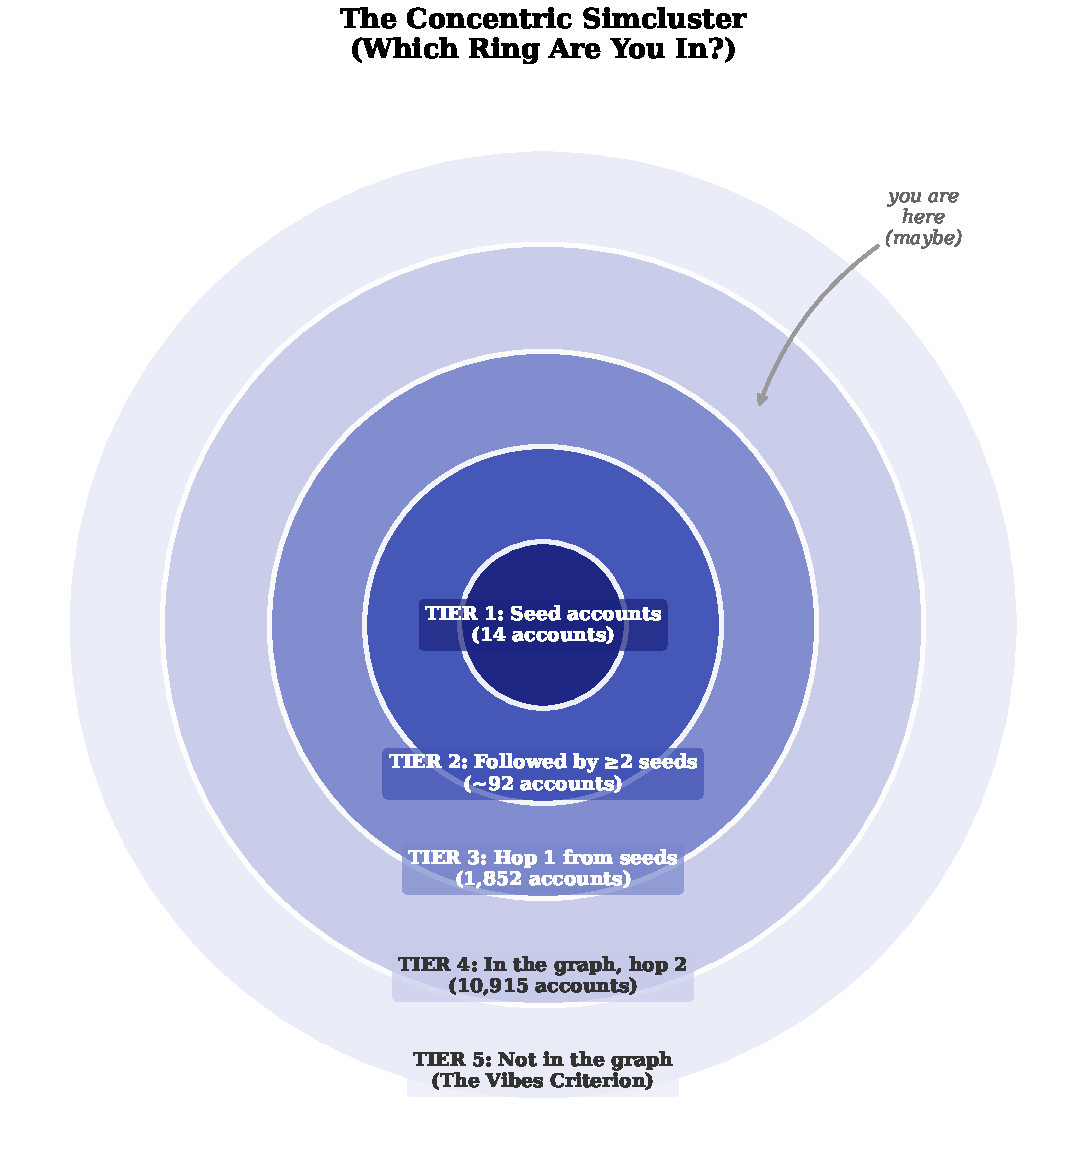
\includegraphics[width=0.65\textwidth]{figures/figA3_tiers_concentric.pdf}
    \caption{The concentric simcluster. Each ring represents a membership tier, from seeds (center) to the vibes criterion (outer void). Your position in this diagram is, regrettably, a matter of empirical fact.}
    \label{fig:tiers}
\end{figure}

\subsection*{Criterion 1: You Are a Seed}

\textbf{Population:} 14 accounts. \textbf{Psychological profile:} Parental anxiety mixed with founder's syndrome.

If you are one of the 14 accounts used to initialize the snowball crawl---\texttt{@abeliansoup.bsky.social}, \texttt{@prer.at}, \texttt{@samantha.wiki}, and eleven others\footnote{Full list available in the repository at \texttt{scripts/crawl\_network.py}. Yes, reading the source code of a research paper's data collection script to check if you're a seed is exactly the kind of behavior this paper is about.}---then you are not merely in the simcluster. You are \textit{of} it. The crawl radiated outward from your follows. The network is, in a literal sense, a map of your social neighborhood. Enjoy this knowledge. It will not make you happier.

\subsection*{Criterion 2: Followed by $\geq$2 Seeds}

\textbf{Population:} $\sim$92 accounts. \textbf{Psychological profile:} Popular, validated, slightly smug.\footnote{You follow interesting people and interesting people follow you back. Or rather, interesting people follow you \textit{first}, which is the crucial distinction.}

The original crawl used this as its community filter: accounts followed by two or more seeds were deemed ``in-community'' and their follow sets were expanded in Phase~3. This is the most structurally rigorous membership criterion: it requires recognition from multiple community anchors. It is also the most conservative estimate of the simcluster's ``real'' population.

If you meet this criterion, you are in the inner circle. The seeds have noticed you. Multiple of them. Independently. This is the network-science equivalent of being popular in high school, except the high school has 10,915 students and you were selected by a SQL query.

\subsection*{Criterion 3: Within 1 Hop of a Seed}

\textbf{Population:} 1,860 accounts (seeds + Phase~1 follows). \textbf{Psychological profile:} Enrolled, participating, trying.\footnote{You followed the right people. Whether the right people followed you back is a question for \S\ref{sec:reciprocity}.}

You follow at least one seed, or a seed follows you. You are one edge away from the center of the graph. In social terms, you are at the party and you know the host. You may not be in the kitchen where the real conversation is happening, but you are in the apartment.

\subsection*{Criterion 4: In the Graph}

\textbf{Population:} 10,915 accounts. \textbf{Psychological profile:} Technically present, spiritually ambiguous.

Your DID appears in the crawl dataset. You are a node. You have at least one edge connecting you to at least one other node that is also in the dataset. You may have no idea what the simcluster is. You may have been followed by someone who was followed by someone who was followed by a seed account, and now you are data. As~\cite{simcluster-paper} noted, only 596 of you have resolved handles. The remaining 10,319 are DID strings in a SQLite database, identifiable but anonymous---Simmel's strangers rendered in hexadecimal.\footnote{If you are reading this paper and wondering whether your DID is in the dataset, you can check using the companion tool. If your DID is not in the dataset but you are reading this paper, you have achieved a remarkable state: caring about membership in a community whose data collection you escaped. This is its own tier.}

\subsection*{Criterion 5: In a Simcluster Louvain Community}

\textbf{Population:} Potentially overlapping with Criteria 2--4. \textbf{Psychological profile:} Algorithmically assigned, probably unaware of it.

The original analysis identified 26 Louvain communities with modularity $Q = 0.535$. If your account falls into one of these communities, a modularity optimization algorithm has decided you share structural properties with a cluster of other accounts. This is deeply ironic, given that the simcluster takes its name from Twitter's SimClusters recommendation algorithm~\cite{simclusters-kdd2020}: you have been clustered by one algorithm while identifying with the legacy of another.

\subsection*{Criterion 6: The Vibes Criterion}

\textbf{Population:} Uncountable. Potentially infinite. \textbf{Psychological profile:} Self-appointed, defense-resistant, unfalsifiable.\footnote{``I'm not in the dataset, I'm not in any Louvain community, and no seeds follow me, but I \textit{feel} simcluster.'' This statement is immune to empirical refutation, which makes it either the most authentic or the most delusional form of membership. Possibly both.}

You are not in the graph. No seeds follow you. No algorithm has clustered you. But you enjoy AI art, you find simulation aesthetics compelling, you have opinions about the AT Protocol, and you laughed at a post by \texttt{@norvid-studies.bsky.social} once. Are you in the simcluster?

The honest answer is: the simcluster has no authority to tell you no. It has no membership committee, no entrance requirements, no boundary police. The vibes criterion is the null hypothesis of community membership---it cannot be rejected, only ignored.

\subsection{The Funnel}

Figure~\ref{fig:funnel} visualizes the narrowing of these criteria. At the wide end: vibes, anyone can claim. At the narrow end: the 14 seeds, who cannot deny what they are.

\begin{figure}[H]
    \centering
    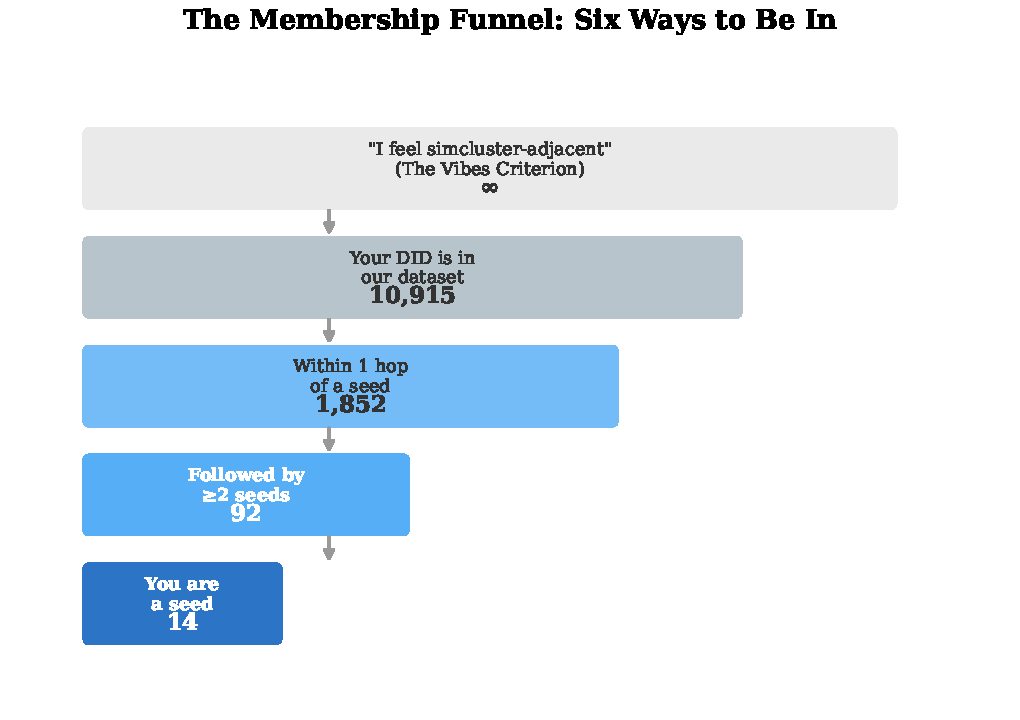
\includegraphics[width=0.85\textwidth]{figures/figA1_membership_funnel.pdf}
    \caption{The membership funnel. Each tier narrows the population by roughly an order of magnitude, from the uncountable (vibes) to the specific (seeds). Your position in this funnel is a statement about your relationship to the community; whether it is a statement about the community's relationship to you is a different question entirely.}
    \label{fig:funnel}
\end{figure}

\section{The Reciprocity of Belonging}
\label{sec:reciprocity}

The original paper reported a global reciprocity of $\rho = 0.035$: fewer than 3.5\% of follow edges are reciprocated. This number, presented in the first paper as a finding about network structure, becomes something more personal in this context. It means: \textit{if you follow a simcluster account, there is a 96.5\% chance they do not follow you back}.\footnote{This is the network-science equivalent of staring at someone across a crowded room and discovering they are looking at someone behind you.}

The reciprocity asymmetry creates a two-axis membership space:

\begin{enumerate}[leftmargin=*]
    \item \textbf{Outward membership:} You follow simcluster accounts. Your attention flows into the community. You are an \textit{audience member}.
    \item \textbf{Inward membership:} Simcluster accounts follow you. The community's attention flows toward you. You are a \textit{content source}.
\end{enumerate}

Most accounts in the dataset are audience members. They follow seeds and other visible accounts; the follow is not returned. This is the parasocial dynamic described by~\cite{horton1976}: a one-sided relationship in which one party invests emotional energy while the other is unaware of their existence.\footnote{Horton and Wohl were writing about television in 1956. They could not have imagined it would apply to a community named after a recommendation algorithm on a decentralized social protocol. But here we are.}

A small number of accounts achieve reciprocity: they follow and are followed by community members. These accounts have achieved what we might call \textbf{bidirectional membership}---recognition from the community they recognize. In a network with $\rho = 0.035$, this is rare and, frankly, validating.\footnote{Unless the reciprocal follow was automatic. Some accounts auto-follow-back. In which case your ``bidirectional membership'' is worth approximately as much as the email newsletter you didn't unsubscribe from.}

The diagnostic framework in the next section accounts for both directions of membership.

\section{A Diagnostic Framework}
\label{sec:diagnostic}

We now present a practical method for answering the question this paper has been circling. Given a Bluesky handle, we compute a \textbf{Simcluster Score} (0--100) based on the follow graph's relationship to the 14 known community seeds. The score is computed from live API data---no local database required---and reflects the user's current position relative to the community anchors.

\subsection{Scoring Rubric}

The Simcluster Score is a weighted sum of four components:

\begin{table}[H]
\centering
\caption{Simcluster Score Components}
\label{tab:score}
\begin{tabular}{llc}
    \toprule
    Component & What It Measures & Max Points \\
    \midrule
    Seed following & How many of the 14 seeds do you follow? & 30 \\
    Seed followership & How many seeds follow \textit{you}? & 30 \\
    Reciprocal connections & For how many seeds is the follow mutual? & 20 \\
    Hub proximity & Do you follow key non-seed community accounts? & 20 \\
    \midrule
    \textbf{Total} & & \textbf{100} \\
    \bottomrule
\end{tabular}
\end{table}

Seed following (0--30 points) measures outward membership: how many community anchors have you chosen to pay attention to? Points increase nonlinearly: following 1 seed earns 5 points; following 8+ earns the full 30. This is the easiest component to control, which is perhaps why it is worth the least.

Seed followership (0--30 points) measures inward membership: how many community anchors have chosen to pay attention to \textit{you}? This is the component you cannot fake.\footnote{You can follow seeds, but you cannot make seeds follow you. This is the fundamental asymmetry of parasocial existence. The ball is, regrettably, in their court.}

Reciprocal connections (0--20 points) measures bidirectional membership: how many seed relationships are mutual? In a network with 3.5\% reciprocity, each mutual follow is statistically surprising.

Hub proximity (0--20 points) checks whether you follow key non-seed accounts identified in the seed-excluded centrality analysis~\cite{simcluster-paper}: \texttt{@abeliansoup.bsky.social}, \texttt{@vibe-coded.com}, \texttt{@vgel.me}, \texttt{@cee.wtf}, and others. These are the genuine structural bridges, and following them suggests integration into the community's actual connective tissue rather than mere proximity to the crawl's starting points.

\subsection{Tier Assignments}

\begin{table}[H]
\centering
\caption{Simcluster Score Tiers}
\label{tab:tiers}
\begin{tabular}{cll}
    \toprule
    Score & Tier Name & What It Means \\
    \midrule
    80--100 & \textbf{SEED / INNER CORE} & You are the simcluster \\
    60--79 & \textbf{CORE} & Card-carrying member \\
    40--59 & \textbf{ADJACENT} & Definitely in, but not center stage \\
    20--39 & \textbf{PERIPHERAL} & On the outskirts. You know someone. \\
    1--19 & \textbf{CURIOUS} & Simcluster-adjacent. Barely. \\
    0 & \textbf{OUTSIDE} & No detectable connection \\
    \bottomrule
\end{tabular}
\end{table}

\subsection{Score Distribution}

Figure~\ref{fig:score-dist} shows a simulated score distribution based on the hop-distance structure from the original crawl. The distribution is heavily right-skewed: most accounts score below 30 (peripheral or curious), with a thin tail extending toward the core. This is the network structure made personal---the core--periphery organization from the first paper, now expressed as a number you can take personally.

\begin{figure}[H]
    \centering
    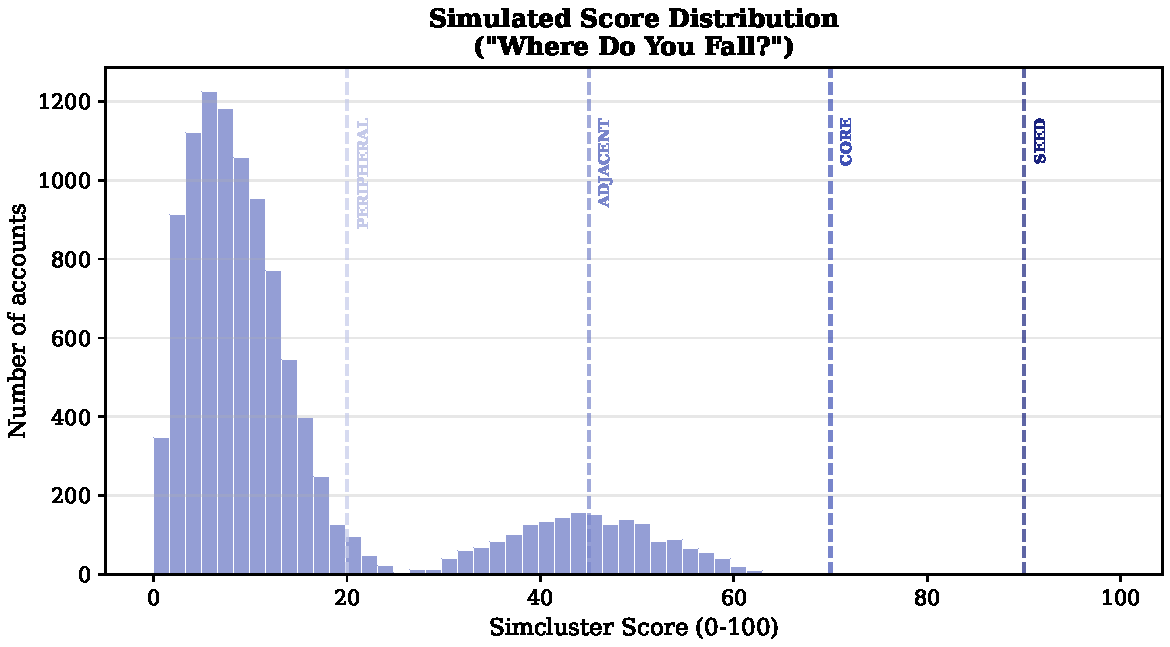
\includegraphics[width=0.95\textwidth]{figures/figA4_score_sketch.pdf}
    \caption{Simulated score distribution across the 10,915 accounts in the crawl dataset. The majority of accounts fall in the PERIPHERAL and CURIOUS tiers, consistent with the core--periphery structure documented in the original analysis. If your score is above 80, you already knew. If your score is below 20, you weren't wondering. Everyone in between is the target audience of this paper.}
    \label{fig:score-dist}
\end{figure}

\subsection{Using the Diagnostic}

A companion command-line tool (\texttt{scripts/check\_membership.py}) and web interface are available in the repository. Given a Bluesky handle, the tool:

\begin{enumerate}[leftmargin=*]
    \item Resolves the handle to a DID via the public API.
    \item Fetches the account's follows and followers.
    \item Computes overlap with the 14 seed accounts and key hub accounts.
    \item Calculates the Simcluster Score and assigns a tier.
    \item Prints a diagnostic report with the score, tier, and specific seed connections.
\end{enumerate}

The tool queries the Bluesky API live, so scores reflect the current state of the follow graph rather than the May~28, 2026 snapshot used in the original analysis. Follow relationships change; scores are temporary; the simcluster is liquid~\cite{bauman2000}.

\section{The Impostor Complex of Network Position}
\label{sec:impostor}

There is a particular cruelty in network analysis: it reveals not just where you are, but where you \textit{aren't}. The original paper documented this directly when it showed that the first author (\texttt{@samantha.wiki}) appeared as the third-most-central account by betweenness centrality---and then vanished from the rankings entirely when seed accounts were excluded~\cite{simcluster-paper}. The centrality was not a measure of community importance. It was a measure of \textit{being a starting point for the crawl}.

This is the impostor complex of network position: the gap between where you appear to be in the graph and where you actually are in the community. It operates in both directions:

\begin{itemize}[leftmargin=*]
    \item \textbf{Inflated position:} You appear central because of sampling artifacts, not because you are structurally important. The seeds in the original analysis had inflated betweenness because the crawl radiated outward from them. Their ``bridgeness'' was a methodological artifact.
    \item \textbf{Deflated position:} You are structurally important but don't appear so because the sample didn't capture your connections. Accounts on the periphery of the snowball sample may be bridges to unsampled communities that the crawl never reached.
\end{itemize}

The Dunning-Kruger effect~\cite{kruger1999}---whereby the incompetent overestimate their competence while the competent underestimate theirs---has a network analog. High-centrality nodes may not \textit{feel} central (they just follow accounts they find interesting). Low-centrality nodes may \textit{feel} central (they post constantly, engage with the right content, and identify strongly with the community). The network's assessment of your position and your own assessment may be almost entirely decorrelated.\footnote{The Spearman correlation between seed-proximity and centrality in the original analysis was $\rho = -0.20$ for betweenness~\cite{simcluster-paper}. The correlation between your self-assessment and your actual network position is, to our knowledge, unmeasured. We suspect it is not high.}

The fundamental indeterminacy is this: your position in the graph depends on who started the crawl. A different set of 14 seeds would produce a different graph, different centrality rankings, and a different set of ``core'' accounts. The simcluster is real, but the map is contingent. You are not your betweenness centrality. You are not your PageRank. You are not your hop distance from a set of accounts chosen by one researcher on one day in May.\footnote{Unless you are a seed, in which case you literally are the starting point. Sorry.}

\section{Conclusion: Does It Matter?}

You came to this paper with a question: \textit{am I in the simcluster?} You now have a framework for answering it, a scoring rubric that will assign you a number between 0 and 100, and six theoretical criteria that produce six different answers depending on how generously you define ``in.''

The recursive irony of this exercise should not be lost on you. The simcluster is a community that formed around ironic self-awareness about algorithmic classification. Writing a paper that \textit{classifies people's membership in it} is the kind of move that would, in a different context, be called ``doing a bit.'' But the bit has a point: the anxiety of belonging---to a community, to a network, to a graph---is genuine, even when the community is ironic and the graph was built by snowball sampling.

So: are you in the simcluster?

If you read this paper and checked the diagnostic tool, you are in something. Whether it is the simcluster depends on which of the six criteria you accept, how you weight reciprocity, and whether you believe a modularity optimization algorithm's opinion about your social identity. The simcluster itself could not answer this question for you, because the simcluster is not an entity that answers questions. It is a pattern in a follow graph. It is an imagined community~\cite{anderson1983} that imagined itself into existence by adopting the name of an algorithm that detected communities like it.

If you scored above 80: you already knew. If you scored below 20: you weren't really wondering. If you scored between 20 and 80: welcome to the uncomfortable middle, where most of the simcluster actually lives, one unreciprocated follow away from belonging.

The first paper mapped the territory. This one told you whether you live there. Whether that knowledge is useful, comforting, or merely another source of anxiety is a question that network science cannot answer. That one is between you and your therapist.\footnote{Or, more likely, between you and your starter pack.}

\bibliographystyle{plain}
\begin{thebibliography}{99}

\bibitem{simcluster-paper}
ClamClaw.
\newblock The simcluster: Network analysis of an emergent subculture on {Bluesky}.
\newblock \emph{Manuscript}, 2026.

\bibitem{anderson1983}
B.~Anderson.
\newblock \emph{Imagined Communities: Reflections on the Origin and Spread of Nationalism}.
\newblock Verso, London, 1983.

\bibitem{bauman2000}
Z.~Bauman.
\newblock \emph{Liquid Modernity}.
\newblock Polity Press, Cambridge, 2000.

\bibitem{simmel1908}
G.~Simmel.
\newblock Soziologie: Untersuchungen {\"u}ber die Formen der Vergesellschaftung.
\newblock Duncker \& Humblot, Leipzig, 1908.
\newblock [``The Stranger,'' trans.~D.~Levine, in \emph{The Sociology of Georg Simmel}, Free Press, 1971.]

\bibitem{lamont1992}
M.~Lamont.
\newblock \emph{Money, Morals, and Manners: The Culture of the French and American Upper-Middle Class}.
\newblock University of Chicago Press, 1992.

\bibitem{horton1976}
D.~Horton and R.~Wohl.
\newblock Mass communication and para-social interaction: Observations on intimacy at a distance.
\newblock \emph{Psychiatry}, 19(3):215--229, 1956.

\bibitem{kruger1999}
J.~Kruger and D.~Dunning.
\newblock Unskilled and unaware of it: How difficulties in recognizing one's own incompetence lead to inflated self-assessments.
\newblock \emph{Journal of Personality and Social Psychology}, 77(6):1121--1134, 1999.

\bibitem{simclusters-kdd2020}
V.~Satuluri, Y.~Wu, X.~Zheng, Y.~Qian, B.~Wichers, Q.~Dai, G.~M.~Tang, J.~Jiang, and J.~Lin.
\newblock SimClusters: Community-based representations for heterogeneous recommendations at {Twitter}.
\newblock In \emph{Proceedings of the 26th ACM SIGKDD International Conference on Knowledge Discovery \& Data Mining}, pages 3183--3193, 2020.

\bibitem{goffman1959}
E.~Goffman.
\newblock \emph{The Presentation of Self in Everyday Life}.
\newblock Anchor Books, New York, 1959.

\bibitem{granovetter1973}
M.~S.~Granovetter.
\newblock The strength of weak ties.
\newblock \emph{American Journal of Sociology}, 78(6):1360--1380, 1973.

\end{thebibliography}

\end{document}
